\section{Definição}

\begin{frame}[fragile]{Programação Dinâmica}

    \begin{itemize}
        \item A programação dinâmica é um paradigma de solução de problemas que combina
            características dos outros paradigmas
        \pause

        \item Assim como o paradigma guloso, ela tenta, a cada iteração, optar pela melhor escolha possível
        \pause

        \item Ela também resolve o problema através da combinação das soluções dos subproblemas,
            o que se assemelha à etapa de fusão da divisão e conquista
        \pause

        \item De forma semelhante a busca completa, ela avalia todas as alternativas disponíveis
            igualmente
        \pause

        \item Ela, porém, difere dos demais paradigmas porque evita recalcular um subproblema
            múltiplas vezes por meio da técnica da memorização, e por optar por uma ou mais 
            alternativas apenas após avaliar todas elas
    \end{itemize}

\end{frame}

\begin{frame}[fragile]{Características da programação dinâmica}

    \begin{itemize}
        \item A programação dinâmica é aplicável em problemas que possuem duas características:
        \pause

        \begin{enumerate}
            \item subestrutura ótima (a solução do problema pode ser formada a partir das soluções
                ótimas dos subproblemas); e
        \pause
            \item subproblemas repetidos (problemas compartilham subproblemas em comum).
        \end{enumerate}
        \pause

        \item Caso a segunda característica não esteja presente, não há necessidade de memorização
            e o algoritmo será equivalente a uma busca completa
        \pause

        \item Como a solução do problema será formada a partir da solução dos subproblemas, esta
            solução pode ser descrita por meio de uma relação de recorrência
        \pause

        \item Os subproblemas que não podem mais serem subdivididos e que são necessários para
            a solução dos demais constituem os casos-base do problema
    \end{itemize}

\end{frame}

\begin{frame}[fragile]{Características da programação dinâmica}

    \begin{itemize}
        \item Tanto o problema quanto os subproblemas são caracterizados por estados, os quais
            correspondem ao conjunto de variáveis (e seus respectivos valores) que identificam
            unicamente uma instância do problema
        \pause
        
        \item Uma transição corresponde a relação entre uma instância do problema e os 
            subproblemas necessários à sua solução
        \pause

        \item A complexidade dos algoritmos de programação dinâmica, em geral, é dada pelo
            produto do número total de estados pelo custo das transições de cada estado
        \pause

        \item A dificuldade de aplicação da programação dinâmica, em geral, reside em se determinar
            a relação de recorrência que caracteriza a solução
    \end{itemize}

\end{frame}

\begin{frame}[fragile]{Exemplo de aplicação de programação dinâmica: Números de Fibonacci}


    \begin{itemize}
        \item Considere o problema de se determinar o $n$-ésimo número de Fibonacci
        \pause

        \item Os números de Fibonacci são definido como
        \[
            F(n) = \left\{ \begin{array}{ll}
                    0,& \mbox{se}\ n = 0 \\
                    1,& \mbox{se}\ n = 1 \\
                    F(n - 1) + F(n - 2),& \mbox{caso contrário}
                \end{array}\right.
        \]
        \pause

        \item Esta definição permite uma implementação direta de busca completa, com complexidade
            $O(2^n)$:

            \inputsyntax{cpp}{codes/fib.cpp}

    \end{itemize}

\end{frame}

\begin{frame}[fragile]{Visualização da chamada $F(5)$}

    \begin{figure}
        \centering

        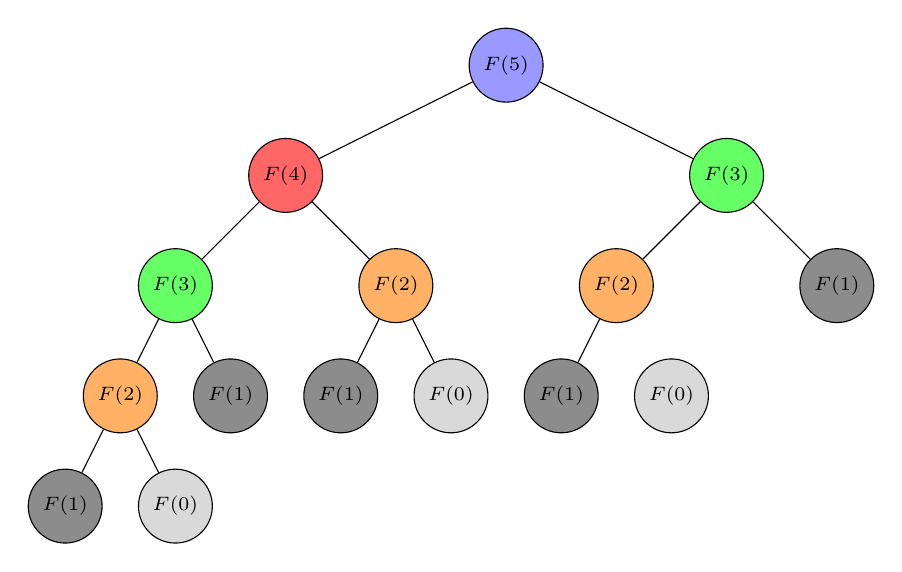
\begin{tikzpicture}[scale=0.7]
            \node[draw,circle,fill=blue!40] (A) at (6, 6) { \scriptsize $F(5)$ };
            \node[draw,circle,fill=red!60] (B) at (2, 4) { \scriptsize $F(4)$ };
            \node[draw,circle,fill=green!60] (C) at (10, 4) { \scriptsize $F(3)$ };
            \node[draw,circle,fill=green!60] (D) at (0, 2) { \scriptsize $F(3)$ };
            \node[draw,circle,fill=orange!60] (E) at (4, 2) { \scriptsize $F(2)$ };
            \node[draw,circle,fill=orange!60] (F) at (8, 2) { \scriptsize $F(2)$ };
            \node[draw,circle,fill=gray!90] (G) at (12, 2) { \scriptsize $F(1)$ };
            \node[draw,circle,fill=orange!60] (H) at (-1, 0) { \scriptsize $F(2)$ };
            \node[draw,circle,fill=gray!90] (I) at (1, 0) { \scriptsize $F(1)$ };
            \node[draw,circle,fill=gray!90] (J) at (3, 0) { \scriptsize $F(1)$ };
            \node[draw,circle,fill=gray!30] (K) at (5, 0) { \scriptsize $F(0)$ };
            \node[draw,circle,fill=gray!90] (L) at (7, 0) { \scriptsize $F(1)$ };
            \node[draw,circle,fill=gray!30] (M) at (9, 0) { \scriptsize $F(0)$ };
            \node[draw,circle,fill=gray!90] (N) at (-2, -2) { \scriptsize $F(1)$ };
            \node[draw,circle,fill=gray!30] (O) at (0, -2) { \scriptsize $F(0)$ };

            \draw (A) edge (B);
            \draw (A) edge (C);
            \draw (B) edge (D);
            \draw (B) edge (E);
            \draw (C) edge (F);
            \draw (C) edge (G);
            \draw (D) edge (H);
            \draw (D) edge (I);
            \draw (E) edge (J);
            \draw (E) edge (K);
            \draw (F) edge (L);
            \draw (H) edge (N);
            \draw (H) edge (O);

        \end{tikzpicture}

    \end{figure}

\end{frame}


\begin{frame}[fragile]{Números de Fibonacci e Programação Dinâmica}

    \begin{itemize}
        \item A figura anterior ilustra a complexidade exponencial da implementação
            apresentada
        \pause

        \item A medida que a recursão avança, alguns estados são computados repetidas vezes
        \pause

        \item Observe que o problema tem subestrutura ótima: o $n$-ésimo número de Fibonacci pode
            ser computado a partir de números de Fibonacci anteriores
        \pause

        \item A repetição de estados com subestrutura ótima o torna um candidato natural para um
            algoritmo de programação dinâmica
        \pause

        \item Com a adição da memorização, a complexidade muda para $O(N)$, um ganho significativo
            de performance
    \end{itemize}

\end{frame}

\begin{frame}[fragile]{Implementação dos números de Fibonacci com PD}
    \inputsnippet{cpp}{1}{20}{codes/fib_td.cpp}
\end{frame}

\begin{frame}[fragile]{Implementação dos números de Fibonacci com PD}
    \inputsnippet{cpp}{22}{42}{codes/fib_td.cpp}
\end{frame}

\begin{frame}[fragile]{Visualização da chamada $F(5)$ com PD}

    \begin{figure}
        \centering

        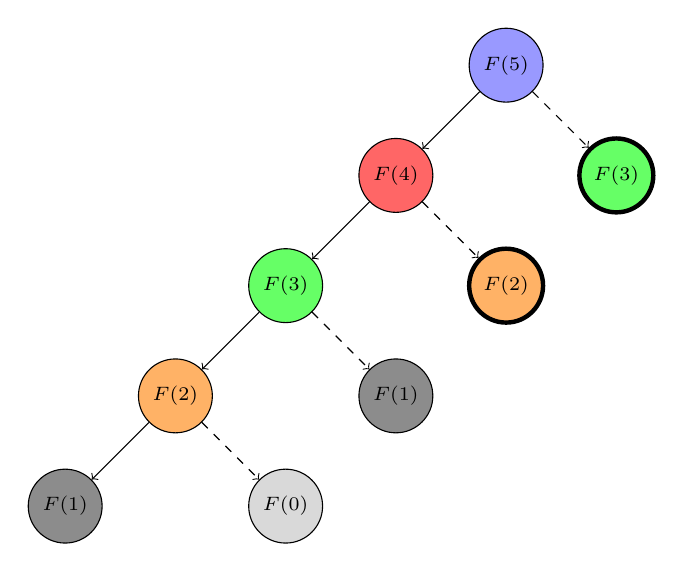
\begin{tikzpicture}[scale=0.7]
            \node[draw,circle,fill=blue!40] (A) at (4, 6) { \scriptsize $F(5)$ };
            \node[draw,circle,fill=red!60] (B) at (2, 4) { \scriptsize $F(4)$ };
            \node[draw,ultra thick,circle,fill=green!60] (C) at (6, 4) { \scriptsize $F(3)$ };
            \node[draw,circle,fill=green!60] (D) at (0, 2) { \scriptsize $F(3)$ };
            \node[draw,ultra thick,circle,fill=orange!60] (E) at (4, 2) { \scriptsize $F(2)$ };
            \node[draw,circle,fill=orange!60] (H) at (-2, 0) { \scriptsize $F(2)$ };
            \node[draw,circle,fill=gray!90] (I) at (2, 0) { \scriptsize $F(1)$ };
            \node[draw,circle,fill=gray!90] (N) at (-4, -2) { \scriptsize $F(1)$ };
            \node[draw,circle,fill=gray!30] (O) at (0, -2) { \scriptsize $F(0)$ };

            \draw[->] (A) edge (B);
            \draw[->,dashed] (A) edge (C);
            \draw[->] (B) edge (D);
            \draw[->,dashed] (B) edge (E);
            \draw[->] (D) edge (H);
            \draw[->,dashed] (D) edge (I);
            \draw[->] (H) edge (N);
            \draw[->,dashed] (H) edge (O);

        \end{tikzpicture}

    \end{figure}

\end{frame}


\begin{frame}[fragile]{Números de Fibonacci e Programação Dinâmica}

    \begin{itemize}
        \item A implementação utilizando programação dinâmica visita cada estado, no máximo,
            duas vezes
        \pause

        \item Na primeira visita (setas contínuas) o estado é computado recursivamente, utilizando
            a mesma recorrência da solução de busca completa
        \pause

        \item Na segunda visita (setas pontilhadas) o estado já foi computado, e o valor armazenado
            na tabela é retornado imediatamente
        \pause

        \item Assim, a complexidade é $O(N)$
        \pause

        \item Observe que, exceto pela memorização e inicialização da tabela, o código é idêntico
            à implementação de busca completa
        \pause

        \item Este tipo de implementação é denominada \textit{top-down}
        \pause

        \item Há uma segunda forma de implementação de algoritmos de programação dinâmica,
            denominada \textit{bottom-up}
    \end{itemize}

\end{frame}
